\documentclass{article}

\usepackage{geometry}
\usepackage{graphicx}
\graphicspath{{./}}

\title{Distributed System\\ Final Report: HTTP over RPC}
\author{Le Nhu Chu Hiep \and Pham Thi Ngoc Mai \and Pham Phan Bach \and Doan Lien Huong \and Vu Khanh Huyen}
\begin{document}
\maketitle
\tableofcontents
\pagebreak
\section{Introduction}
HTTP over RPC is quite a interesting topic. In here, we try
to build the proxy servers that sit between client and its
destination.
\\
\\
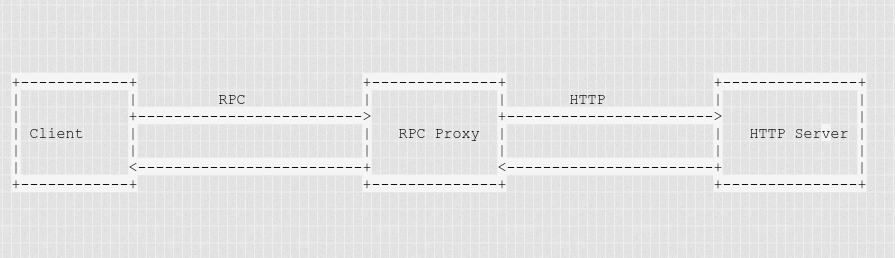
\includegraphics[scale=0.5]{RPC_topic}
\\
\\
In this project, our requirement is that the
client and the proxy will communicate through RPC protocol.
There are 2 ways to understand it:\\
\\
Firstly, the proxy can provide severial HTTP generate
function so that the client can use to send request to
the destination host (Of course the function call in here
is remote - RPC function).
But I think it is not preference way for 2 reason. It is
not productive and the general user can not used.
And the other way will be providing the data transfer proxy
as normal proxy and applying the RPC as the protocol. In
other other word, the client give proxy poorly HTTP as
data and we help them transfer it to destinate. And in
the middle of the line, the RPC protocol will be used.\\
\\
Developing from second idea, the proxy can split out or
we can say it is distributed proxy. Basicaly, there are
2 parts in the proxy system, the bunch of servers will
get the client HTTP request and the other server send request
HTTP to the destination host. The RPC is used as main protocol
between 2 type server of system.\\
\\
Why do we run this project ?\newline Obviously, this is our final
and the sub reason is the knowledge that I can gain about
proxy. And it sound very cool also.
\section{Objective}
My purpose in this project is understand the proxy definition
and use it to develope the runable proxy between the real browser
(in this case is the firefox) and any destination HTTP and HTTPS
host. During building idea time, I decide to implement 2 type server:
\begin{itemize}
\item The client proxy server which stand in the same region as
the client and can have multi-server across each geography space.
It will sit in demo computer for convenient reason. This server type
handle the client request send in as poor HTTP or HTTPS. Parse the
client request to get IP and port of destinate host, talk to other
type server (RPC protocol) to open tunnel between client and 
destination.
\item Other type server in here is the server proxy server. 
It is a bad name (I know). But it is the important part in 
my proxy system. It run outside of the censored region. Waiting
for incomming request of the client server (in RPC protocol).
Creating TCP socket to destination host, then open tunnel between
client and host website. It keep the role as end user in the
website point of view.
\end{itemize}
Note that my browser is firefox 74 so the communication with
client will follow standard of firefox 74 in proxy mode.
\section{State of the art}
Unfortunately, we could not found any the proxy server apply
RPC protocol into the commnucation. It can be explained because
most of the proxy system work as a single station. That mean
the user will send the request to a server and that server itself
sends request to the destination host. That is a simple and easy
implemented method.\\
\\
However, it is lack of security protection when the single location
of the proxy server can be found. Then the middle-man can track out
the client IP to identify the user location. But if the proxy system
are distributed as my idea, even if the part connect to the website
be found, it is still be hard to keep tracking the user IP because
the user dont connect directly to tracked server. Moreover, it is
easier to scale up sysetm. Basicaly, the server proxy part do 1 job
only is transfer data the host website. And the hard part which is
handle request from the user (include multiple of proxy communicate
protocol depending on the browser type and version) stay in the client
proxy server part. Then when the proxy implement
some new feature, instead of closing the wholw system to update,
the new client proxy part will be deployed then connect to on-running
server proxy part. I call it dynamic update
\section{Method}
The result of analysis part can be encapsulate in below picture
\\
\\
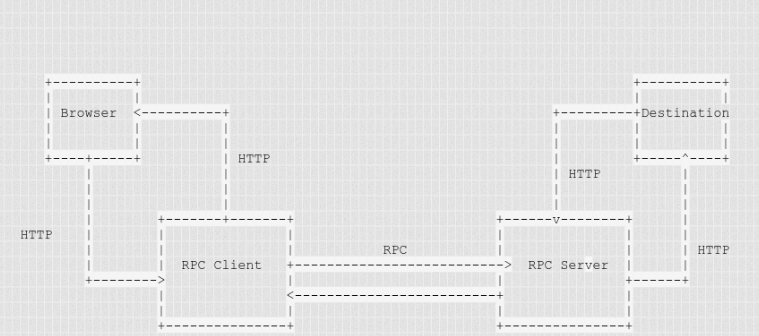
\includegraphics[scale=0.5]{RPC_method}
\\
\\
In this figure, the proxy system will redirect request from the browser
to the destination website through several step.
\begin{enumerate}
\item The browser send request to the RPC client proxy (HTTP protocol)
\item The RPC client parse the request and request new connection to RPC
server proxy (RPC protocol)
\item The RPC server connect to the website as the request from the RPC
client (TCP connection)
\item The RPC client send confirm to the client that the tunnel between
the user and the host is ready
\item The client consider the RPC client as the destination and send
real request (HTTP(s) protocol)
\item The RPC client send that request to RPC server and it read the final
host
\item After the request get response (success or fail), the RPC client send
close request to the RPC server to finalize connection (tunnel close)
\end{enumerate}
For each piece of the proxy system, I apply several definition and technique,
It will be clarified in sub parts below. 
\subsection{Firefox Proxy protocol}
Before we can go furthermore, the definition of the proxy system is important
include what it is and how it work. So basically, a proxy server acts as a
gateway between the user and the internet. Its an intermediary server separating
end users from the websites they browse. Then if the browser use the proxy server,
the internet traffic will flow through the proxy server to the address requested.
After that, the response will return to that proxy server and be forwarded back to
the browser. In this model, the proxy server act as a filter between you and internet.
You can prohibit some unwanted website. Or another better way, the proxy server work
like a firewall help protect you from the internet security attack. But that is
another story.\\
\\
For now, let concentrate on the proxy server operate (in very basic concept).
\begin{enumerate}
\item The client send request "openning tunnel" to the proxy include final host address
\item The proxy open tunnel to the final host and send confirm response to the client.
From now on, any request come from the client will be forward to the final host and vice versa
\item The client begin send HTTP(s) request and get response.
\end{enumerate}
This is quite simple definition of a proxy system. I follow it to deplay my own proxy. But
there was some unpredictable happen. The firefox proxy implementation is not alway follow
all steps. With HTTPS protocol, the step above is correct, browser send "open tunnel" request
by using method "CONNECT" in HTTP. I can gather the host and port of destinate, open tunnel
as define.\\
\\
But in HTTP mode, firefox dont act right, it ignore 2 first step and just send HTTP directly
to the proxy server as in step 3. Of course I can still collect the host and port of destinate,
then open tunnel. But it require the proxy need to be seperated into 2 mode: HTTPS mode and HTTP
mode. This weird action of firefox must be noticed during developement time.
\subsection{Sun Microsystems ONC RPC}
As mention before, This is a disteibuted proxy server. And the communication protocol
between this system is RPC (Remote procedure call). This protocol allow the user call
the execute function on remote machine. It can consider like you split a process into
2 part and push each part to defference device. Therefore, it support the ditributed 
process and be used in many distributed system. I use this protocol for my system because
that is my final ds course topic.\\
\\
RPC is only mechanism, so there are a bunch of implementation. And I use the implement of
Sun Microsystems ONC (it is very popular in the linux system). It provide several tool to
work with RPC. The \textbf{rpcgen} for generate source course and \textbf{rpcbind} to run
server.
\begin{itemize}
\item \emph{"rpcgen"} : it is the RPC protocol compiler from RPC IDL of ONC. It is very
convenient tool when it create not only RPC function and stub but also the example and
makefile in C source code. I can modify the example file to reach my target. Then compile
all with \textbf{make} tool
\item \emph{"rpcbind"} : is utility work as server that converts RPC program number into
universal addresses. It must be runing on the host to be able to make RPC calls on a server
on that machine. When RPC service is started, it tells rpcbind the address at which it is
listening, and the RPC program numbers it is prepared to serve. So basically, you need to 
run this utility to open RPC server on the machine.
\end{itemize}
By the way, talk about the IDL of RPC ONC, it is defined as struct below:
\begin{verbatim}
program name_pro {
  version name_ver {
    return_type name_func(parameter) = func_num;
  } = ver_num;
} = pro_num;
\end{verbatim}
The definition and struct of IDL is well define in official website of ONC.
And you can read my IDL for this project in file has extension *.x
\subsection{TCP socket}
This is a basic and important definition. It keep the main role in the
distributed system (the proxy system in this case). It is an internet endpoint
for sending or receiving data within a node on a computer
network. Whenever the machine
want to communicate with another machine, it need to open network socket.
Then every data transfer between 2 devices will be relate to this socket.
In other word, the network socket help distribute resource among devices in
a network. Then TCP socket is transmission control protocol socket. It lay in
layer transport in OSI model. It keep alive the connection between 2 node in
the network and guarantee the successive of data flow in network from source
to destination. HTTP protocol run on top of TCP protocol.\\
\\
In this project, I use C program TCP socket system call of linux to open listening
port on the RPC client proxy and connect the RPC server proxy to the final website.
And the TCP socket can be create with function
\begin{verbatim}
/* socket system call */

int socket(int domain, int type, int protocol);

/*
* For more information - man(2)
*/
\end{verbatim}
This function will return file descriptor of the network socket.
Then it can be consider as a file in linux system and can be
read, write as normal. In this case, when you read or write, data
instead of storing to file system, it is transfer to the other machine.
\subsection{Fork}
Fork is a system call of linux os. It creates a new process by dyplicating
the calling process. the new process is referred to as the child process.
And the calling process is referred to as the parent process.\\
\\
This system call sit in the RPC client proxy and used to fork 
new process when ever there are new HTTP request come to the server.
I follow the definition of HTTP - it is stateless protocol. That mean
each HTTP request come to the proxy system is unique 
and cannot know the exit of the other request even they go at same time.
For this reason, whenever new HTTP request sent to the proxy, the server
will create a new process only serving that HTTP request. It can be
represent in these steps:
\begin{itemize}
\item Server listens on port A
\item HTTP request sent to server
\item Server accept new connection
\item Server fork new process. Parent keep listening
and child handle HTTP request.
\end{itemize}
There are some worry about the memory space required if the whole server is
forked for each process. But HTTP connection is very short with only 1 request
with 1 response. So the overhead case is very rare.
\subsection{fcntl.h}
This another linux system call. It stand for file control - In this library,
I use only function fcntl(). It perform some operation on open files. In other
word, It can modify some properties of file descriptor. In this case is NONBLOCKING
property.\\
\\
For normal case, when ever the process read to file descriptor,
it is blocked and wait until there are data to read. It is not exception with
network socket which is act as a normal file in the linux space. But when the
proxy server begin run the tunnel mode. The data can flow from 2 direction. The
client to the website and the website back to the client. So if the read function
function is blocked when try to read data from client. But actually, the client
is waiting for the reponse of the website. Then although the website return response.
The proxy server is still be block in read client side. Then it will be dead block case.
The same situation can happen when the server read the website first. Then solution is
very simple, modify properties of file descriptor then push read/write into loop. Then
when the proxy read the client, if it do not have data, it return -1 and jump to read 
the website.
\section{Evaluation}
\subsection{Success}
Up to this report time, the proxy system can handle both HTTP and HTTPS versions.
It can tunnel for a small amount HTTP requests instantaneous. I can tunnel the
www.google.com (HTTPS ver) homepage successful.\\
\\
With HTTP version, the main page of firefox homepage is transfer successful.\\
\\
The time performance is not fast as direct connection but if compare to another proxy
browsec extension of firefox, it is same (Of course because I can verify 2 website test only).
For the mechanism of parsing HTTP header in first step of the proxy protocol. The limitation
for head length should smaller then 500 bytes.
\subsection{Bug}
\begin{itemize}
\item RPC call time out is most bug of the project (I still not have time to find the reason)
\item RPC can not encrypt parameter for RPC call. This bug come from wrong type define in IDL.
In first time, I use string, but that type will end if reaching '\\0' value. Then I change to
char array type. It work well after that but sometimes, the error still appear.
\item Can not close connection to the server site. It is problem of my close connection mechanism.
I find out it when writing this report on fcntl part.
\end{itemize}
\section{Conclusion}
HTTP over RPC is a interesting topic but not popular in community. It can be unreality but give
effort on researching it give me some hints about the distributed proxy system. Actually, this
model can be implemented and deploy for a decade. But with me, that is new and worth the effort.
Although I build the system only 1 night before presenting and 3 days for finishing this report,
I think I gain a huge amount of knowledge about linux system call, socket, fcntl and feel fork 
is a brilliant idea. There are several bug in the system, I will fix it and keep developing this
project as a habit.
\end{document}